\documentclass[aspectratio=169]{beamer}
\providecommand{\lumenpalette}{blue}
\usetheme[palette=\lumenpalette,progressbar=true,sectionpages=true]{lumen}

\title{Reproducing VISAtlas}
\subtitle{An Image-Based Exploration and Query System for Large Visualization Collections}
\date{\today}

\begin{document}

\begin{frame}[plain]
  \titlepage
\end{frame}

\begin{frame}{Motivation}
  \begin{quote}\itshape
    ``The visualization collections are inherently diverse in many perspectives: from different data sources, by different research groups, and in different manners.''
  \end{quote}
  \vskip0.85em
  \begin{quote}\itshape
    ``Existing systems for visualization images \dots\ are mainly based on extrinsic attributes including author names and publication years.''
  \end{quote}
  \vskip0.85em
  \begin{quote}\itshape
    ``More importantly, attribute-based systems neglect the intrinsic property, i.e., visual appearance of visualizations that is also perceived by humans.''
  \end{quote}
  \vfill
  {\color{lumenPrimary}\bfseries Although visual appearance is directly perceived by humans, it has often been overlooked as an analyzable property of visualization collections.\par}
  \vskip0.6em
  \begin{flushright}
    \scriptsize Y.~Ye, R.~Huang, W.~Zeng. \emph{VISAtlas}. IEEE TVCG 30(7):3224--3240, 2024.
  \end{flushright}
\end{frame}

\begin{frame}{Research Questions}
  \vfill
  \begin{quote}\itshape
    ``Which visualization collection shall be used?\\
    Are there any similar visualizations in the collection?\\
    What visual features are prominent in a visualization?\\
    What visual features are frequently composited in visualizations?''
  \end{quote}
  \vfill
  {\color{lumenPrimary}\bfseries VISAtlas represents the visual appearance of visualizations as interpretable embeddings, enabling users to explore, compare, and query visualization collections based on visual features rather than only extrinsic metadata.\par}
  \vskip0.6em
  \begin{flushright}
    \scriptsize Y.~Ye, R.~Huang, W.~Zeng. \emph{VISAtlas}. IEEE TVCG 30(7):3224--3240, 2024.
  \end{flushright}
\end{frame}

\begin{frame}{Related Work: Citation Provenance}
  \centering
  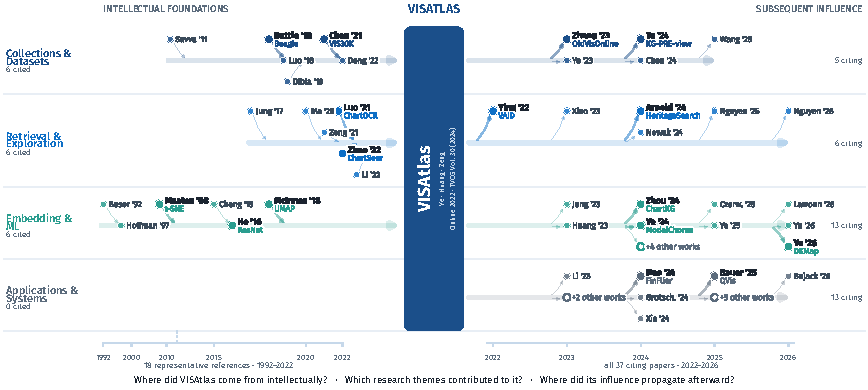
\includegraphics[width=\textwidth]{figures/citation_provenance.pdf}
\end{frame}

\end{document}
